\subsection{An\'alise dos Resultados dos Modelos de Previs\~ao}

A Figura \ref{fig:1-ar} apresenta uma previsão de um passo à frente (um dia). Nos apêndices \ref{sec:ararxma24}, pode-se observar uma comparação entre os modelos AR, MA e ARX.
Todos os modelos de ARIMA e seus antecessores são obtidos pelo método da biblioteca do Python ``autoARIMA''. Mesmo sendo obtidos parâmetros um pouco distintos dos apresentados aqui e usados nos dados, foi feito um ajuste para que os parâmetros tenham os melhores resultados. Foram utilizados os parâmetros obtidos pelo autoARIMA, que são $(p = 6, d = 0, q = 3) (P = 2, D = 1, Q = 0)_{M = 12}$, mas foram ajustados para obter um melhor resultado, sendo $(p = 7, d = 1, q = 7) (P = 2, D = 1, Q = 1)_{M = 12}$ para a média de 24 horas. Na Tabela \ref{tab:autoarima_params}, são exibidos todos os modelos obtidos por esse método do ``autoARIMA'' e ajustados para que obtenham o melhor resultado.
\(p\): Ordem do componente AR (\textit{Auto-Regressivo}),
\(d\): Número de diferenciações não sazonais,
\(q\): Ordem do componente MA (\textit{Média Móvel}),
\(P\): Ordem do componente AR sazonal,
\(D\): Número de diferenciações sazonais,
\(Q\): Ordem do componente MA sazonal,
\(M\): Período sazonal (número de observações em um ciclo sazonal).
Na Tabela \ref{tab:autoarima_params} é exibido como cada modelo ficou.


\begin{table}[tb]
	\centering
	\caption{Parâmetros utilizados nos modelos AR, ARX, MA, ARMA, ARIMA, ARIMAX, SARIMA e SARIMAX obtidos pelo ``autoARIMA'' do Python.}
	\label{tab:autoarima_params}
	\small
	\begin{tabular}{cp{9cm}p{2cm}}
		\hline
		\textbf{Modelo} & \textbf{Parâmetros Utilizados} & \textbf{Método de Estimação} \\
		\hline
		AR(p) & \( p = 7 \) & AutoARIMA do Python \\
		ARX(p) & \( p = 7 \) & AutoARIMA do Python \\
		MA(q) & \( q = 7 \) & AutoARIMA do Python \\
		ARMA(p, q) & \( p = 7 \), \( q = 7 \) & AutoARIMA do Python \\
		ARIMA(p, d, q) & \( p = 7 \), \( d = 1 \), \( q = 7 \) & AutoARIMA do Python \\
		ARIMAX(p, d, q) & \( p = 7 \), \( d = 1 \), \( q = 7 \) & AutoARIMA do Python \\
		SARIMA(p, d, q)(P, D, Q) & \( p = 7 \), \( d = 1 \), \( q = 7 \), \( P = 2 \), \( D = 1 \), \( Q = 1 \), \( M = 12 \) & AutoARIMA do Python \\
		SARIMAX(p, d, q)(P, D, Q, M) & \( p = 7 \), \( d = 1 \), \( q = 7 \), \( P = 2 \), \( D = 1 \), \( Q = 1 \), \( M = 12 \) & AutoARIMA do Python \\
		\hline
	\end{tabular}
	
\end{table}


\begin{figure}[H]
	\centering
	\caption{Comparação dos modelos AR e ARX \label{fig:1-ar} \label{fig:1-arx}}
	\begin{subfigure}{1\textwidth}
		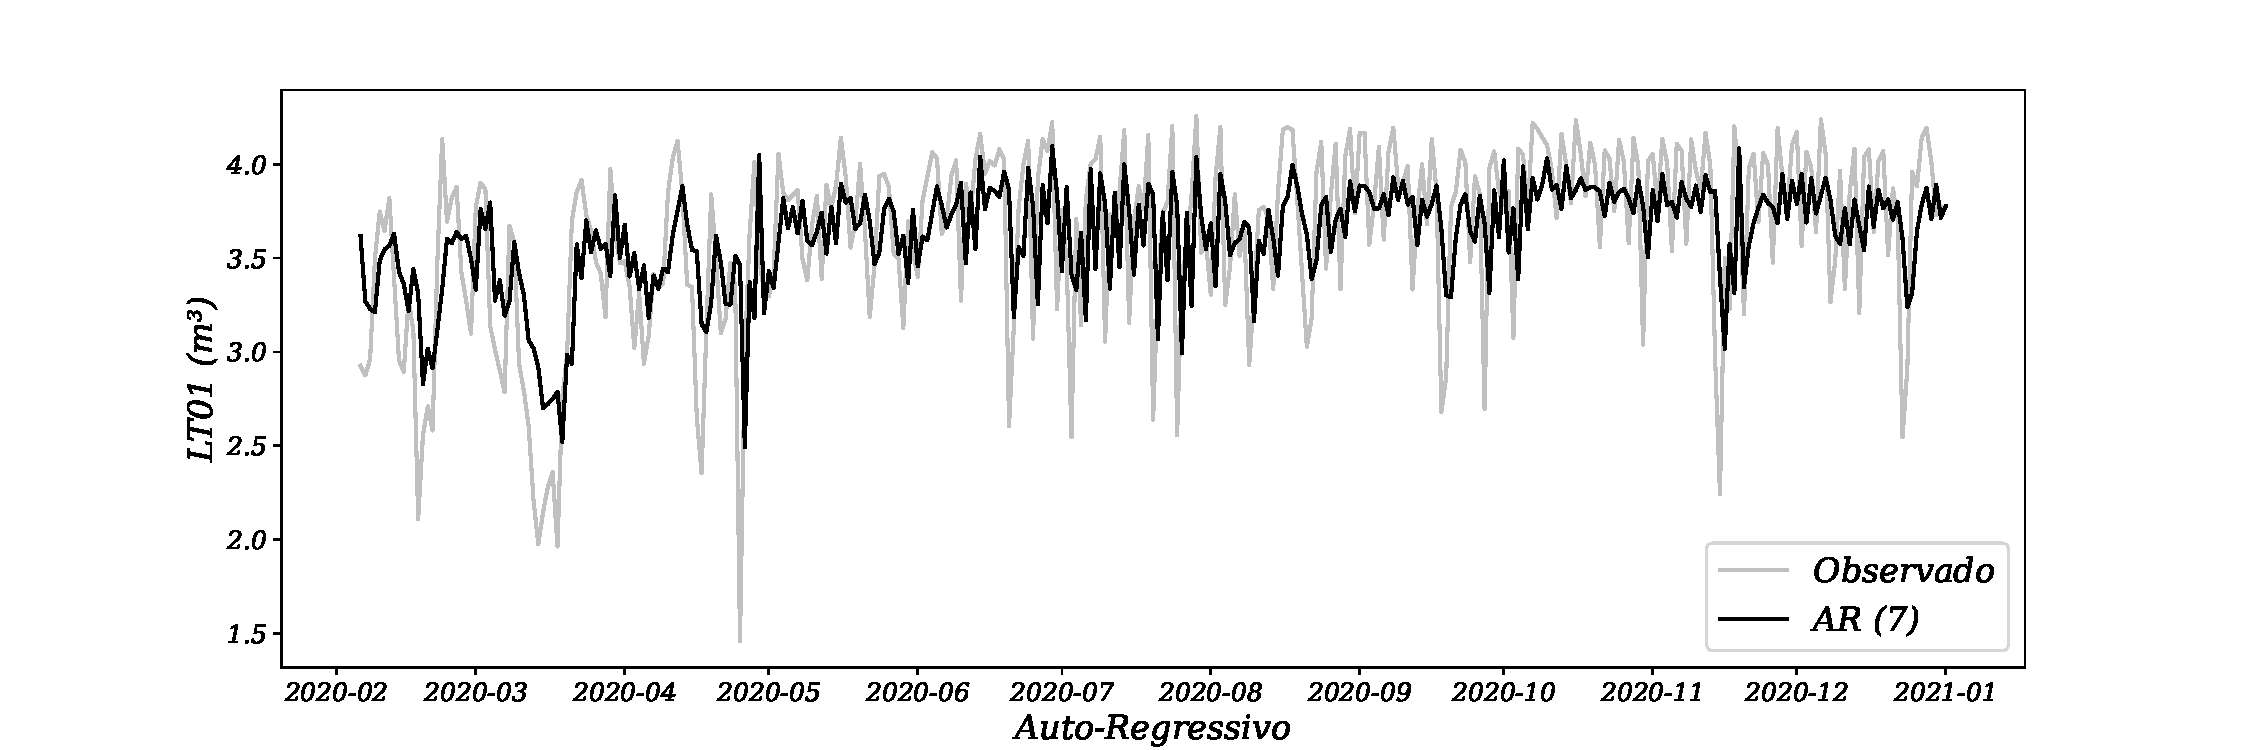
\includegraphics[width=\linewidth]{Modelos/Figuras/AR}
		
		
	\end{subfigure}
	
	\begin{subfigure}{1\textwidth}
		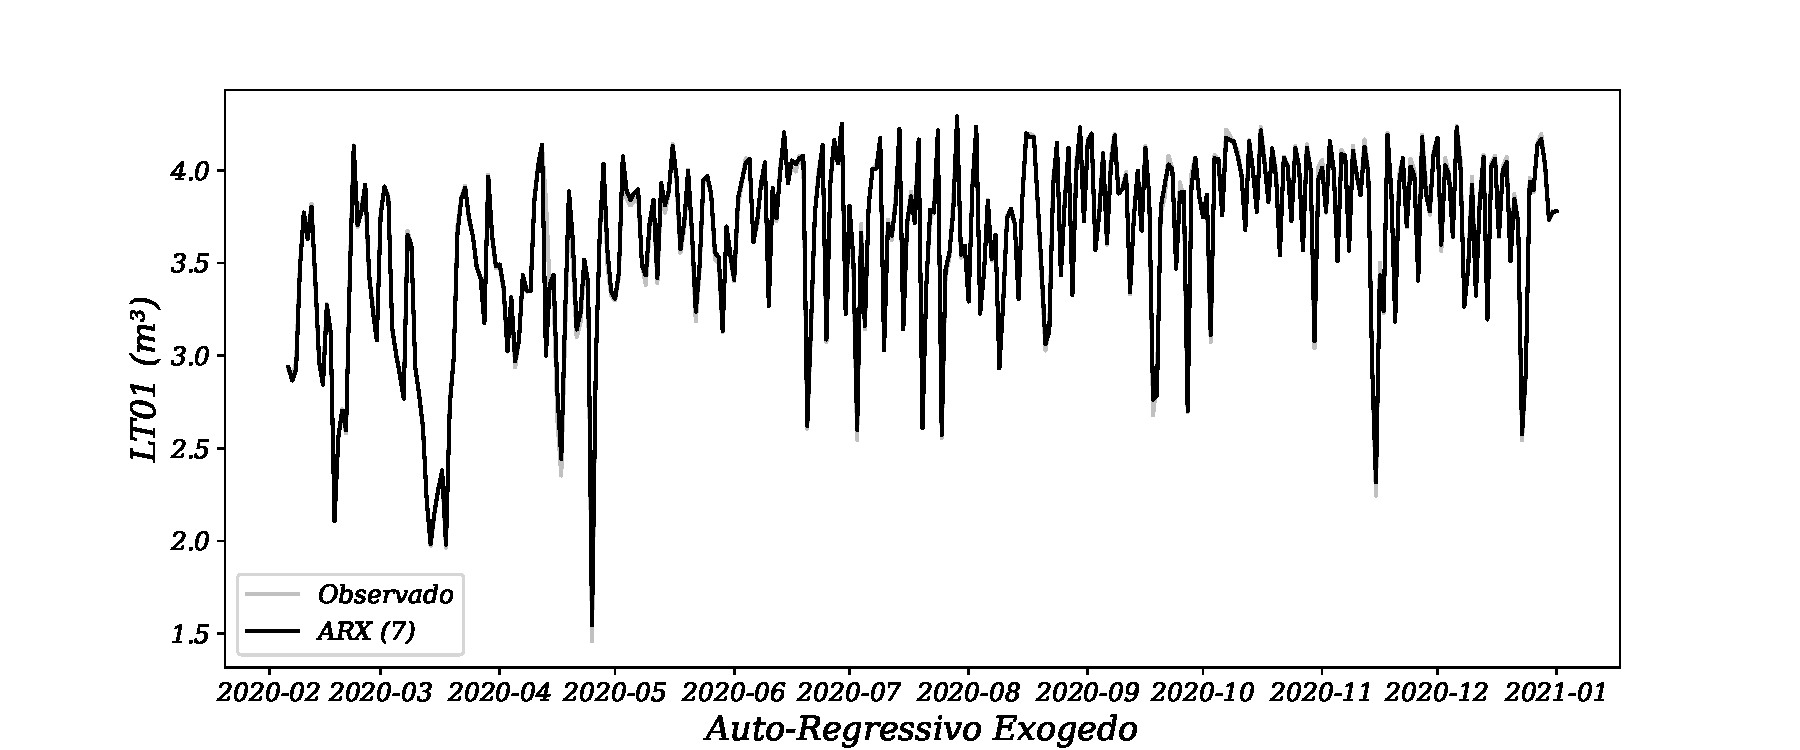
\includegraphics[width=\linewidth]{Modelos/Figuras/ARX}
		
		
	\end{subfigure}
	
	
\end{figure}

O modelo MA, quando comparado com um modelo AR de mesma ordem, gera uma previsão usando o método de médias móveis, enquanto o modelo AR é um modelo regressivo que observa os dados no passado. O modelo MA, por outro lado, observa os erros que esses dados podem cometer. A Figura \ref{fig:1-ma} mostra que essa previsão se assemelha ao modelo apresentado na Figura \ref{fig:1-ar}, embora não seja comparável ao modelo exibido na Figura \ref{fig:1-arx}.

\begin{figure}[H]
	\centering
	\caption{Modelo MA(7) }
	\label{fig:1-ma}
	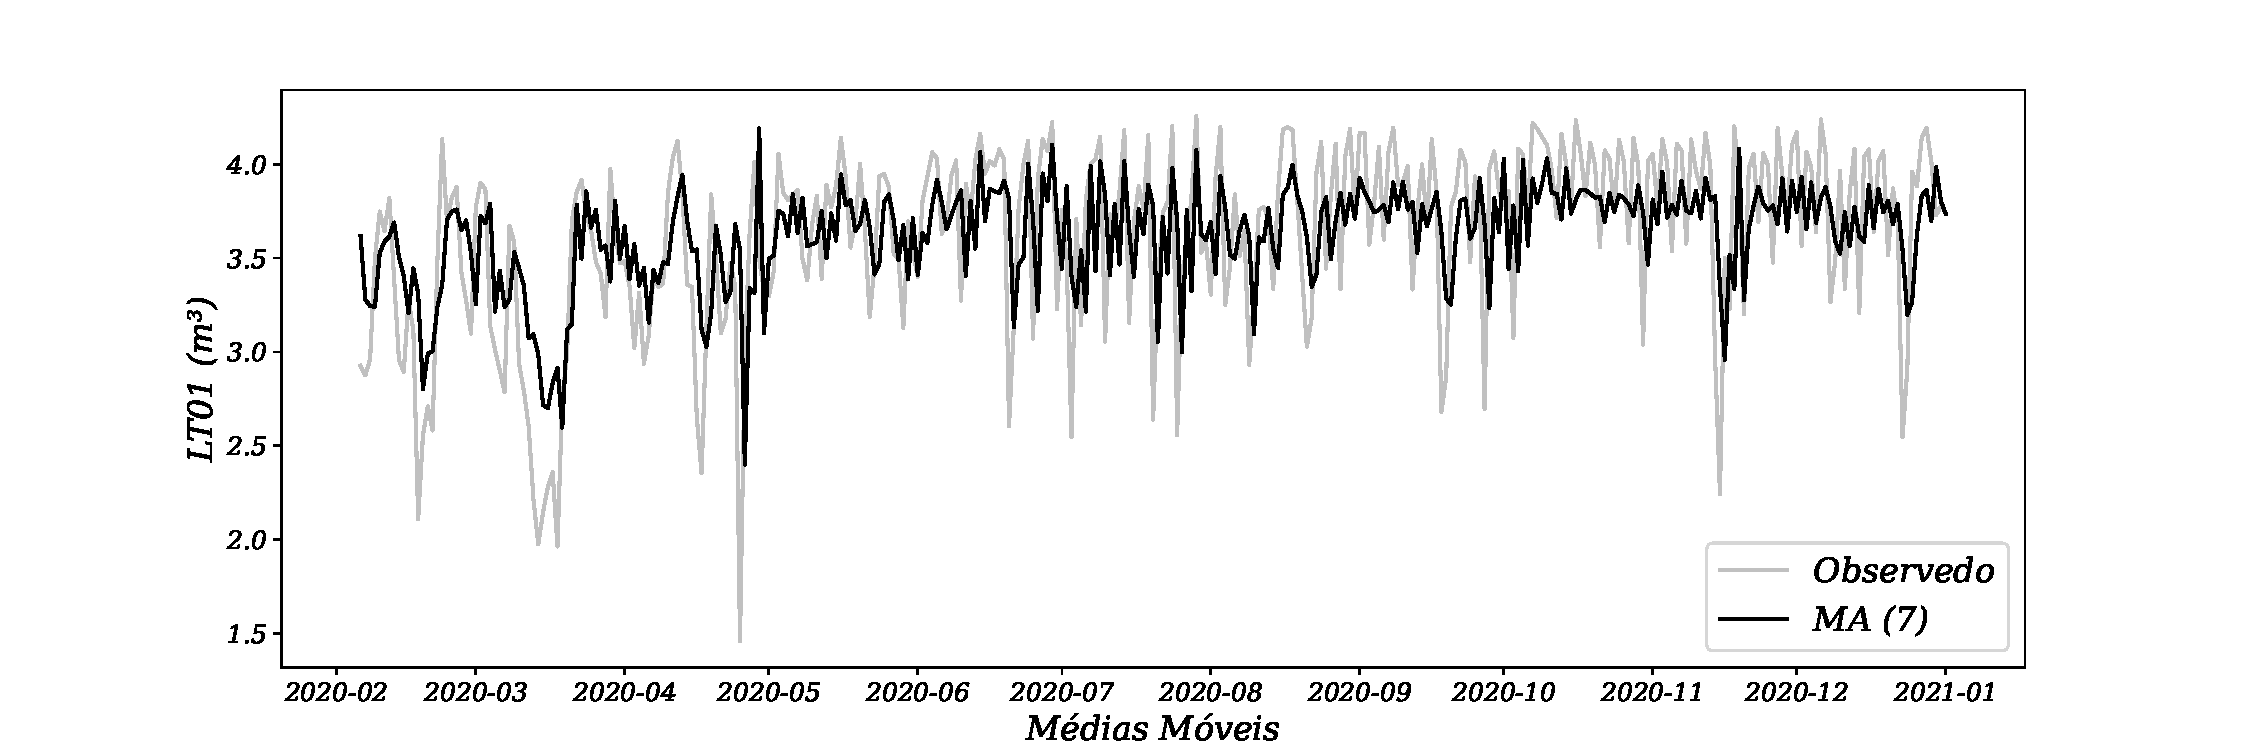
\includegraphics[width=1\linewidth]{Modelos/Figuras/MA}
	
	
\end{figure}

A Figura \ref{fig:1-arma} combina dos modelos AR e MA em um modelo ARMA. Essa abordagem pode levar a uma redução significativa no erro de previsão, como observado nos apêndices \ref{sec:comtb24} e \ref{sec:comtb18}, onde são apresentadas comparações com um número de passos de previsão de 1, 7, 14 e 30 passos à frente.
Ao analisar a Figura \ref{fig:1-arima}, não se nota uma diferença significativa nos erros sMAPE, MAE e RRMSE, conforme indicado no apêndice \ref{sec:comtb24}. Pode-se notar que esta afirmação sugere que os modelos não têm muita diferenciação entre si em comparação com os outros métodos apresentados anteriormente. A análise sugere que o método ARX ainda parece ser superior aos demais.


\begin{figure}[H]
	\centering
	\caption{ARMA (7,7)}
	\label{fig:1-arma}
	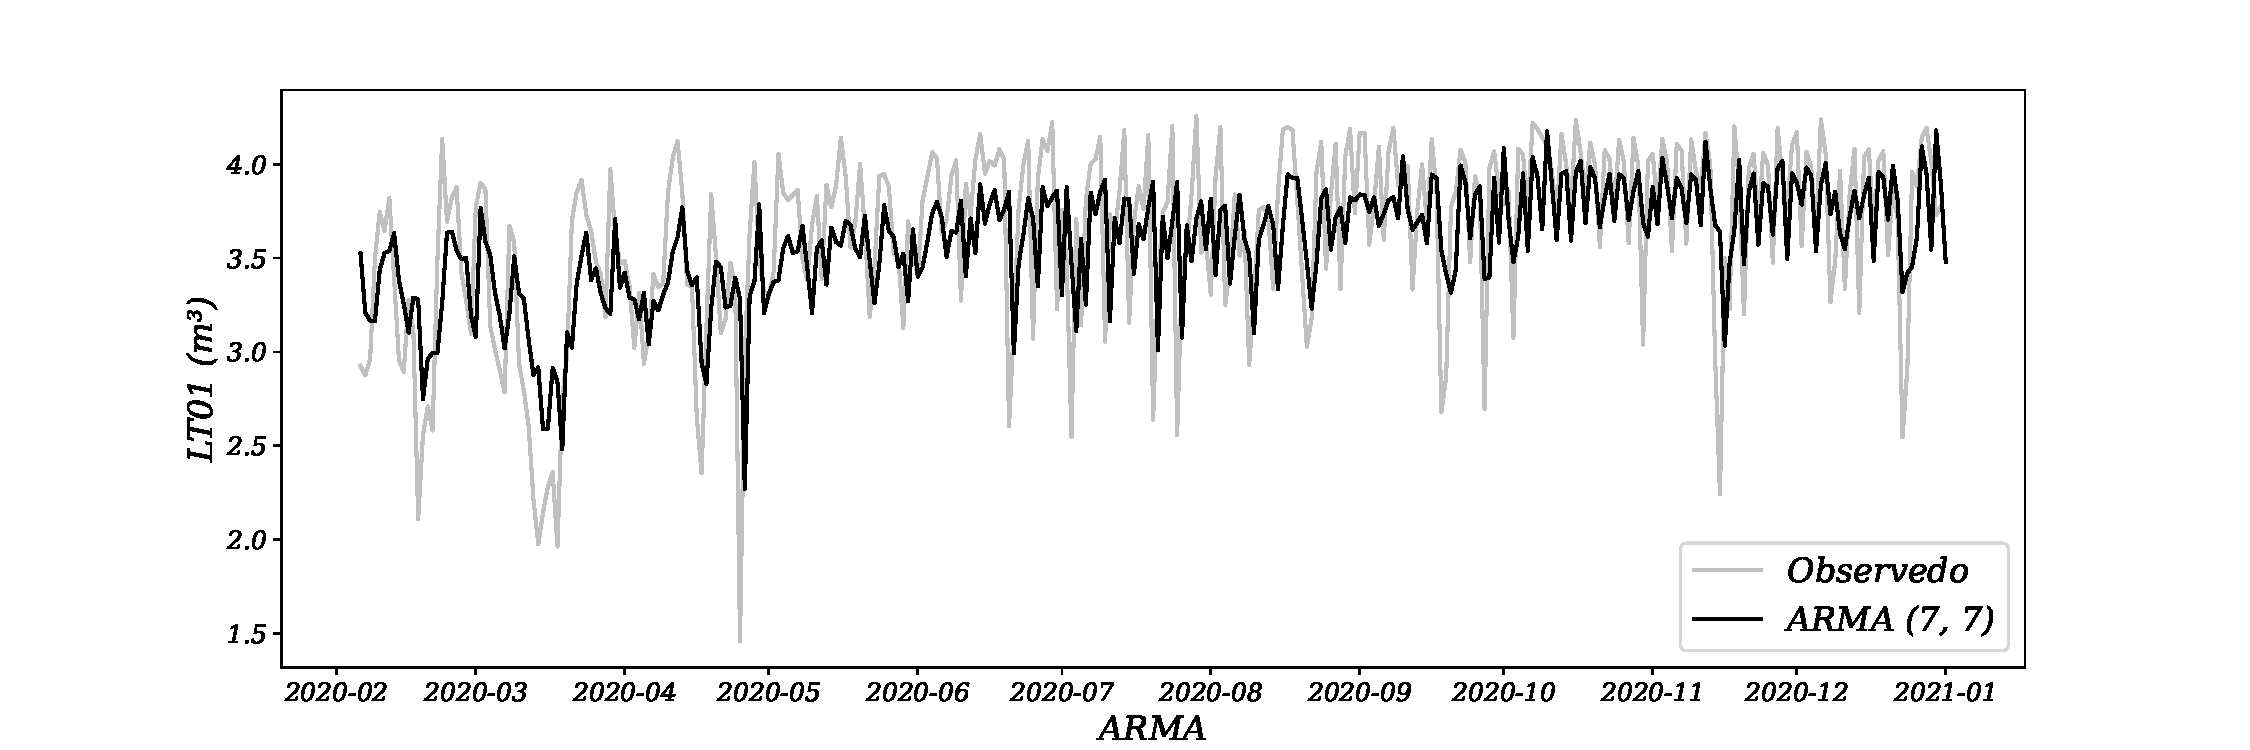
\includegraphics[width=1\linewidth]{Modelos/Figuras/ARMA}
	
	
\end{figure}



\begin{figure}[H]
	\centering
	\caption{ARIMA (7,1,7)}
	\label{fig:1-arima}
	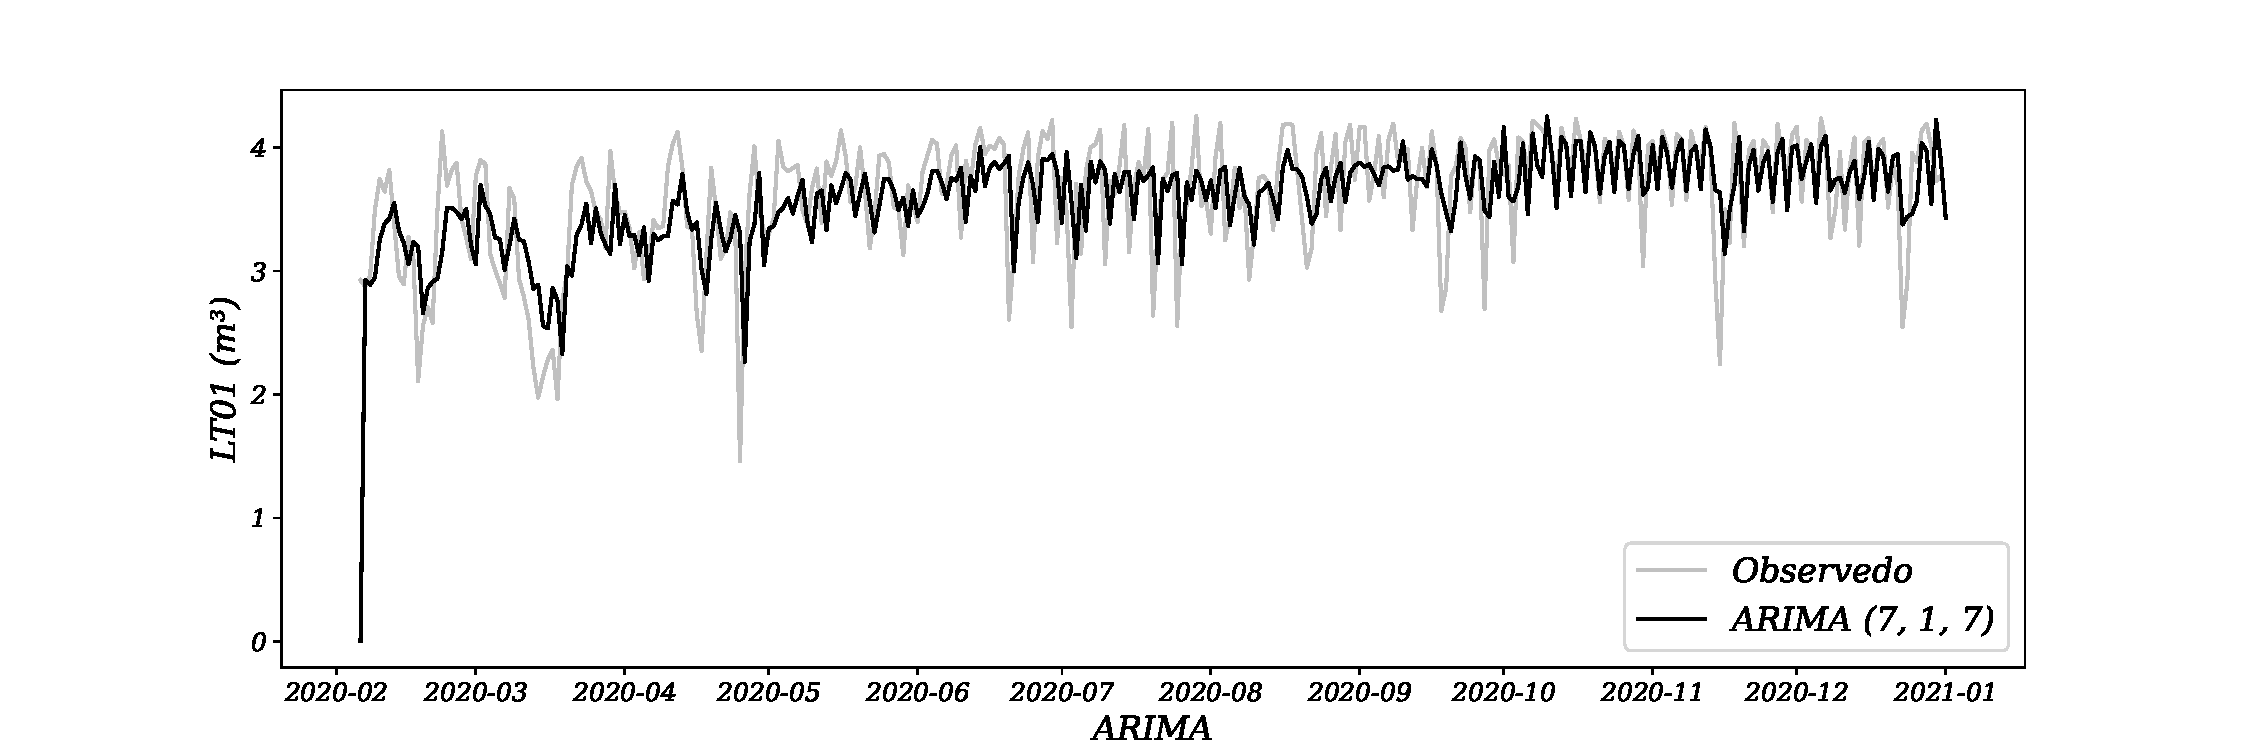
\includegraphics[width=1\linewidth]{Modelos/Figuras/ARIMA}
	
	
\end{figure}


Na Figura \ref{fig:1-sarima}, é possível observar que a previsão em vermelho está próxima dos valores observados em preto, mostrando que a inclusão do componente de sazonalidade melhora a qualidade da previsão. Os modelos SARIMA são capazes de lidar com dados que apresentam padrões sazonais, permitindo a diferenciação dos dados em termos de componentes sazonais e não sazonais. Uma abordagem útil para determinar os melhores parâmetros do modelo é utilizar uma estrutura de pesquisa automatizada de parâmetros, com a biblioteca do Python ``autoARIMA'', que auxilia na identificação dos parâmetros para o modelo SARIMA. 

\begin{figure}[H]
	\centering
	\caption{SARIMA $ (p,q,d)(P,Q,D)=(7,1,7) (2,1,1)_{12}$}
	\label{fig:1-sarima}
	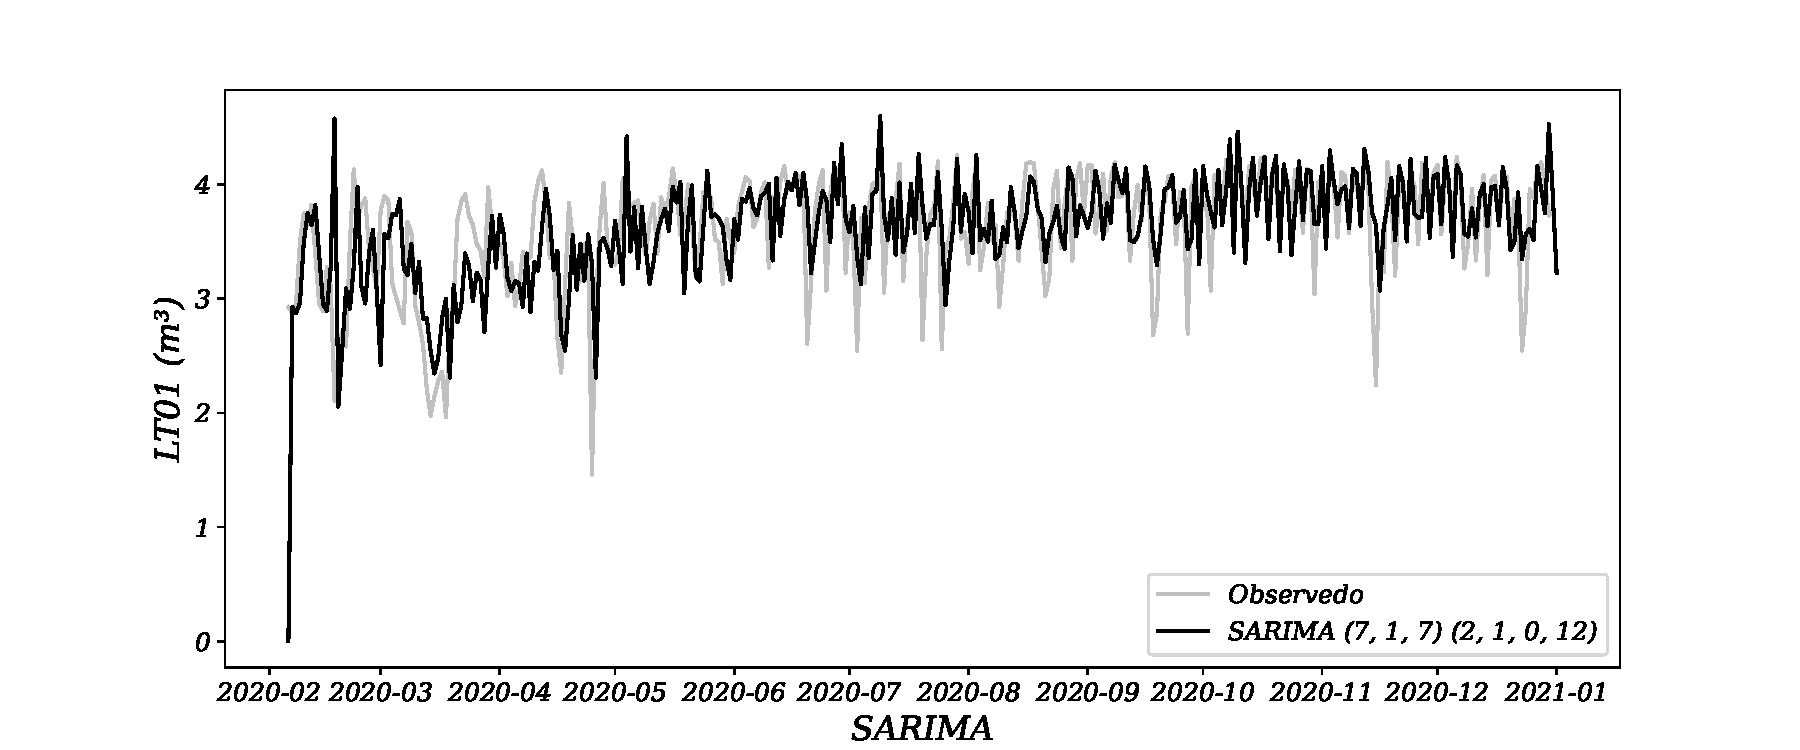
\includegraphics[width=1\linewidth]{Modelos/Figuras/SARIMA}
	
	
\end{figure}

Entre os modelos com variáveis exógenas, como os modelos ARX, ARIMAX e SARIMAX mostrado na Figura \ref{fig:1-arimax}, observa-se uma melhora na qualidade das previsões em comparação com os modelos que não incluem variáveis exógenas. A adição dessas variáveis externas permite capturar melhor a influência e os padrões presentes nos dados, resultando em previsões mais adequadas. Essa inclusão de informações adicionais contribui para uma compreensão mais abrangente do comportamento da série temporal e possibilita uma melhor adaptação do modelo aos padrões observados.

\begin{figure}[H]
	\centering
	\caption{Comparação entre ARIMAX e SARIMAX \label{fig:1-arimax}\label{fig:1-sarimax}}
	\begin{subfigure}{1\textwidth}
		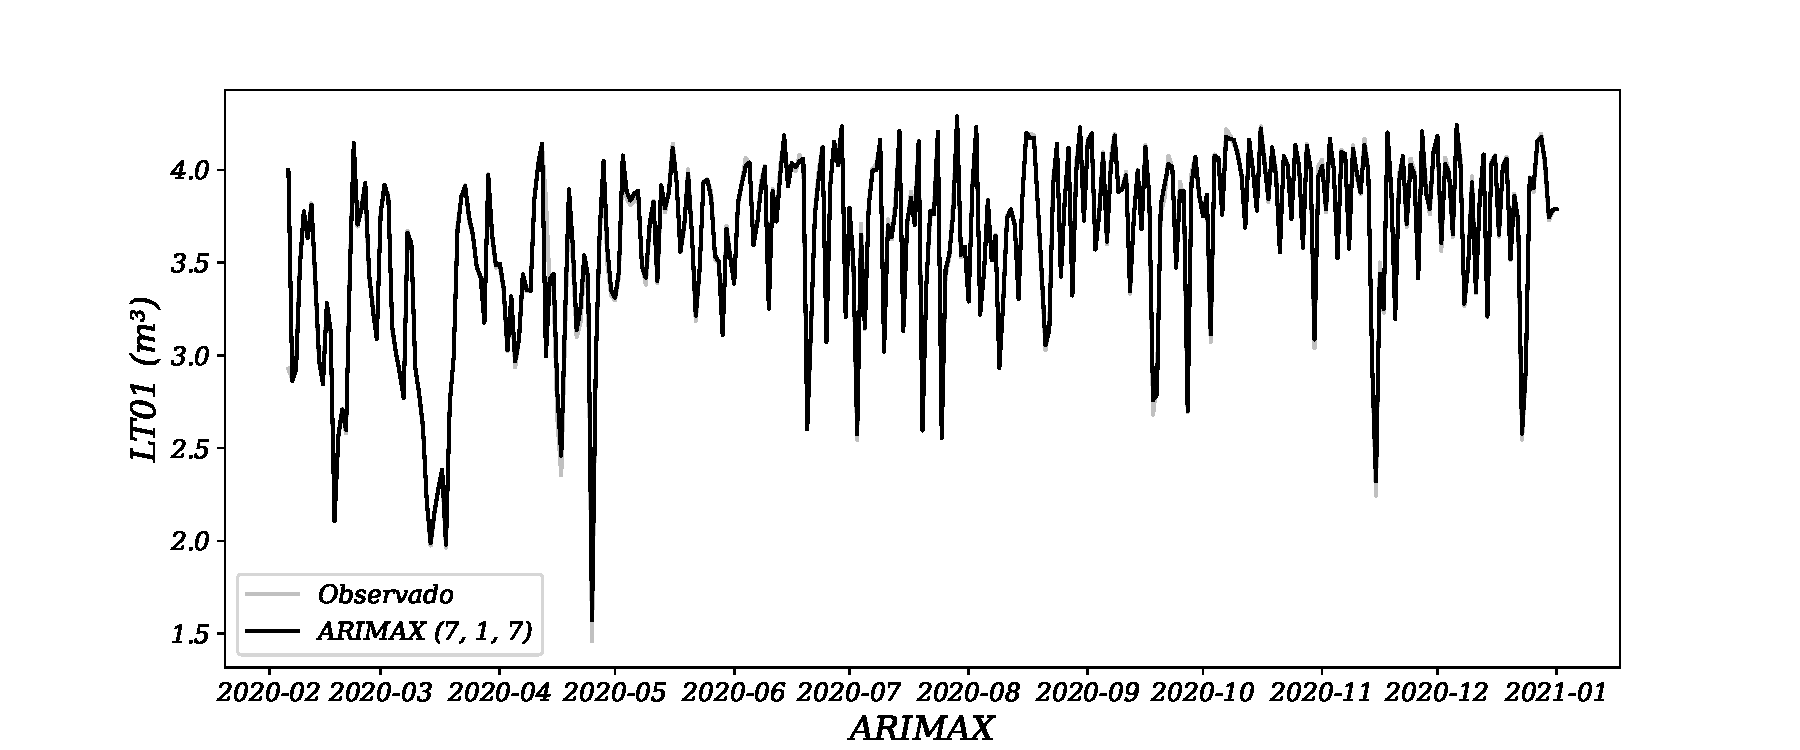
\includegraphics[width=\linewidth]{Modelos/Figuras/ARIMAX}
		
		
	\end{subfigure}
	\hfill
	
	\begin{subfigure}{1\textwidth}
		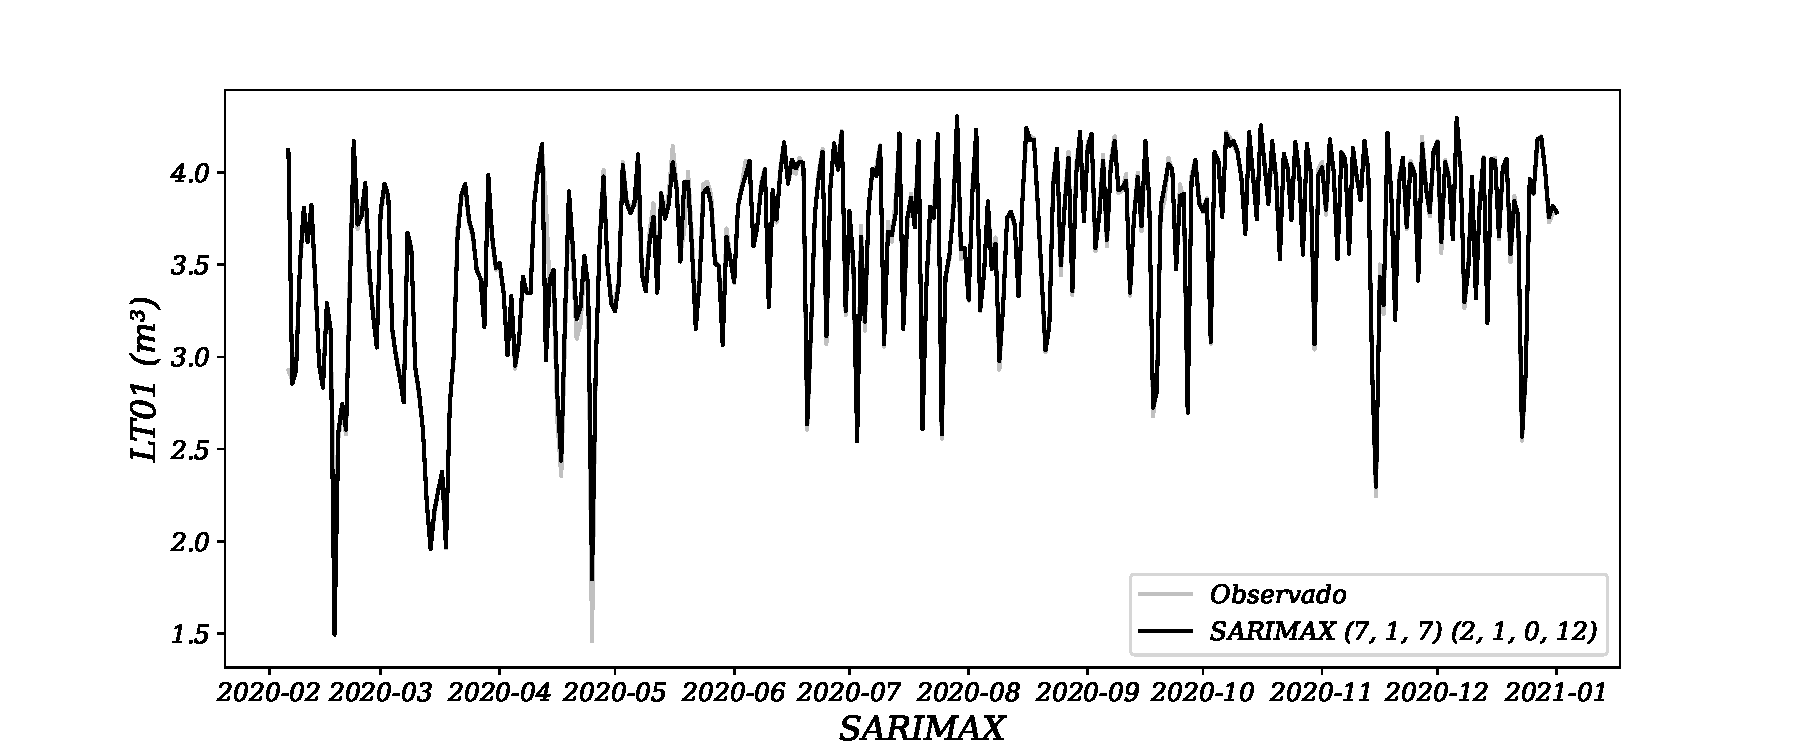
\includegraphics[width=\linewidth]{Modelos/Figuras/SARIMAX}
		
			
	\end{subfigure}
	
	
\end{figure}

Na Figura \ref{fig:prophet1} é apresentada a previsão da variável LT01 usando o Prophet. Este modelo exibe diversas informações, como a sazonalidade dos dados e a tendência. O Prophet é considerado um modelo proposto recentemente que pode ser comparado com ARIMA. 

\begin{figure}[H]
	\centering
	\caption{Previsões do modelo Prophet para o reservatório LT01}\label{fig:prophet1}
	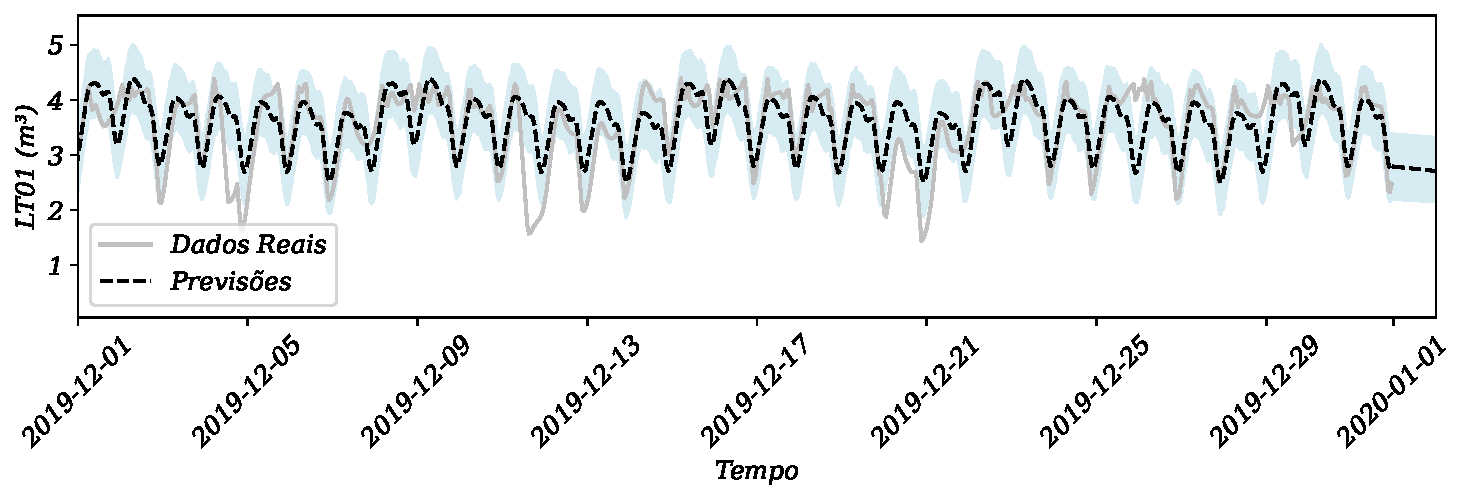
\includegraphics[width=1\linewidth]{Apendices/Figuras/modelagem-24h/prophet1}
	
	
\end{figure}

A Figura \ref{fig:lr-lt01-m3} fornece uma representação dos coeficientes $\beta_0$ e $\beta_1$. Um aumento de $1$ na variável $x$ está associado a um aumento proporcional de $\beta_1$ na variável $y$. O valor de $\beta_0$ representa o valor de $y$ quando $x$ é igual a $0$.

\begin{figure}[H]
	\centering
	\caption{Regressão linear LT01 vs PT01 correlação 98\%}
	\label{fig:lr-lt01-m3}
	\includegraphics[width=1\linewidth]{"Modelos/Figuras/LR LT01 (m³)"}
	
	
\end{figure}

A Figura \ref{fig:1-regressao-linear}, um passo à frente dos dados da SANEPAR foi previsto no modelo LR. Esse modelo mais simples do que os outros modelos pode ser útil em horizonte menor, mas em horizontes de vários dias à frente o desempenho do modelo é degradado. Ele é um dos modelos que apresenta erros acentuados na análise das métricas sMAPE, MAE e RRMSE.

\begin{figure}[H]
	\centering
	\caption{Regressão linear (LR) um passo a frente}
	\label{fig:1-regressao-linear}
	\includegraphics[width=1\linewidth]{Modelos/Figuras/regressão-linear}
	
	
\end{figure}

A Figura \ref{fig:decision-tree-regressor}, é apresentado este modelo com o intuito de diminuir o erro de previsão que o LR estava tendo em prever mais de um dia à frente. Este modelo, por ser mais robusto, consegue trabalhar na otimização dos hiperparâmetros, tornando-o melhor que o LR na questão de horizontes mais longos.

\begin{figure}[H]
	\centering
	\caption{Regressor de \'Arvore de Decis\~ao }\label{fig:decision-tree-regressor}
	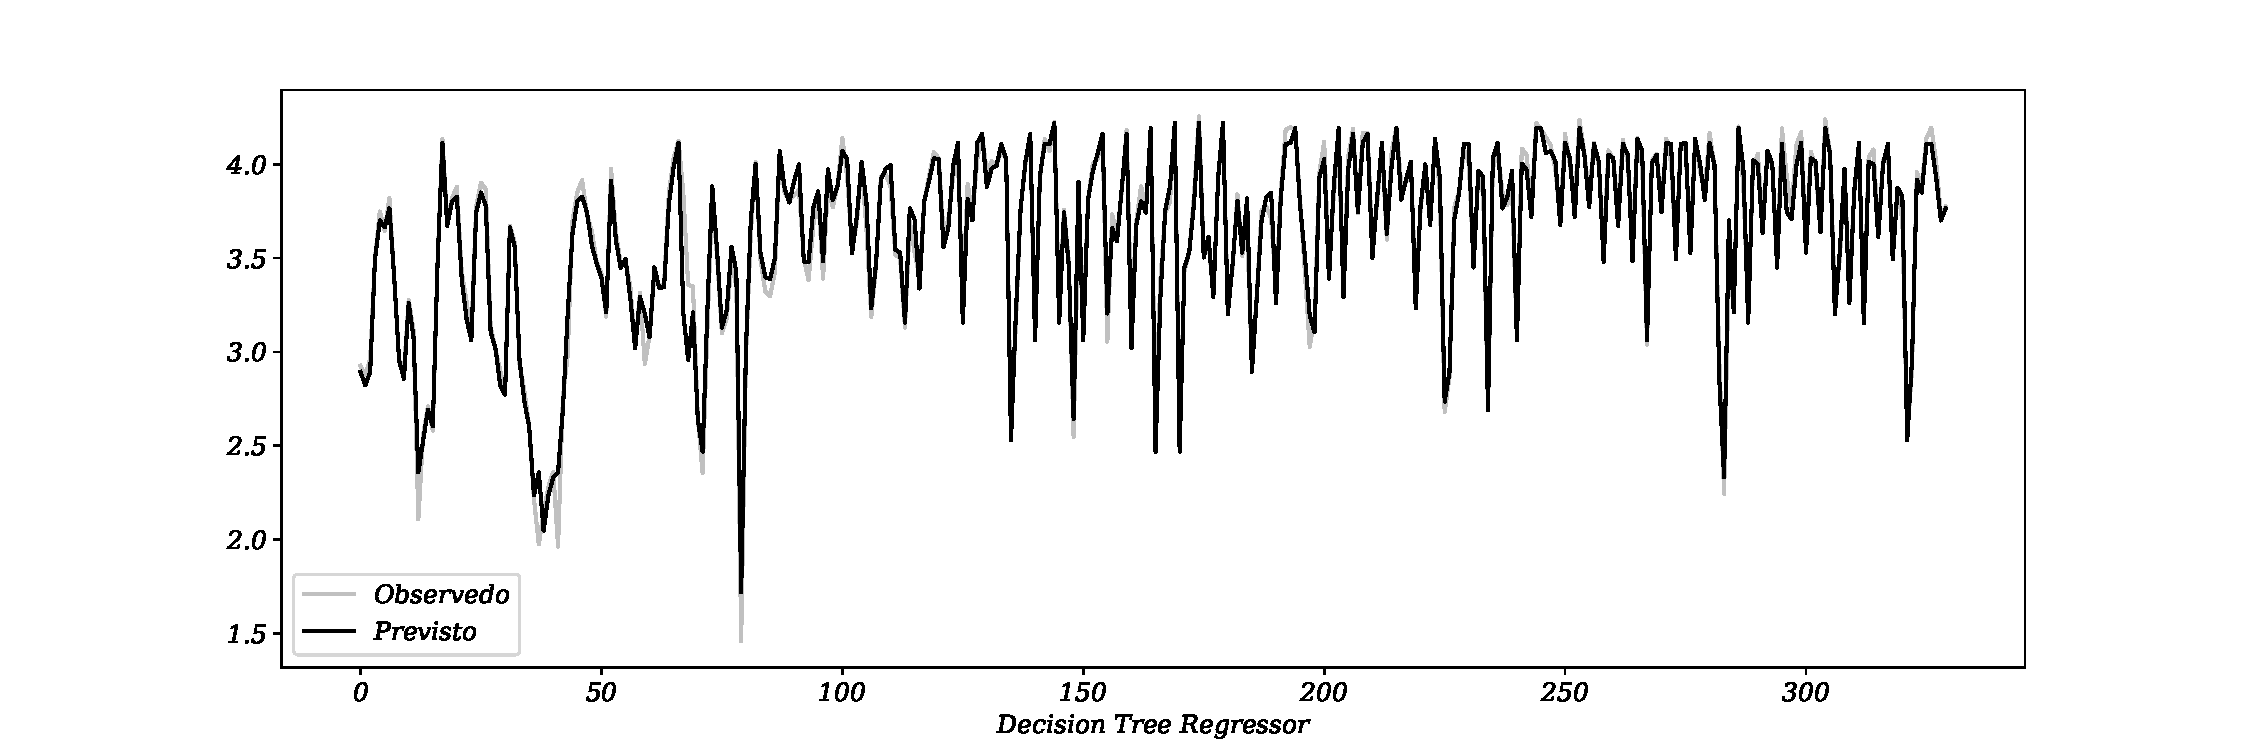
\includegraphics[width=1\linewidth]{Apendices/Figuras/modelagem-24h/Decision-Tree-Regressor}
	
	
\end{figure}

Na Figura \ref{fig:1-regressao-rfa}, o modelo RFR apresentado em comparação com os outros modelos, e ele se destaca em relação aos modelos anteriores já analisados em um passo à frente, mas pelo Tabelas \ref{tb:apd-trn} à \ref{tb:apd-int} pode notar que esse modelo RFR não tem grandes melhores em relação ao outros.


\begin{figure}[H]
	\centering
	\caption{Regressão da Floresta Aleatória (RFR)}
	\label{fig:1-regressao-rfa}
	\includegraphics[width=1\linewidth]{Modelos/Figuras/regressão-rfa}
	
	
\end{figure}

Na Figura \ref{fig:1-xgb-regressao}, são apresentados os modelos XGBoost e LightGBM esses modelos tem como parâmetros e hiperparâmetros obtidos na otimização do Optuna uma biblioteca do Python para otimização de parâmetros e hiperparâmetros como mostrado na Tabela \ref{tab:hiperparametros} a otimização dos paramétrios dos modelos XGBoost, LightGBM, RFR e DTR. Esses modelos, devido à sua semelhança, exibem tempos de desempenho próximos um do outro. Na Figura \ref{fig:xgb}, é exibida uma previsão de um passo à frente, e observa-se que esse modelo parece ser superior aos demais modelos previamente apresentados. Por outro lado, na Figura \ref{fig:lgb}, apesar de ser um modelo mais rápido em termos de tempo de computação, ele ainda não atingiu o desempenho esperado para o tema abordado.



\begin{table}[tb]
	\centering
	\caption{Hiperparâmetros dos modelos}
	\label{tab:hiperparametros}
	\begin{tabular}{p{2.2cm}p{2.8cm}p{1.9cm}p{2cm}p{2cm}p{2cm}p{2cm}}
		\hline
		\textbf{Modelo} & \textbf{Estimadores} & \textbf{Profund. Máxima} & \textbf{Min. Amostras Divisão} & \textbf{Min. Amostras por Folha} & \textbf{Máx. Recursos} & \textbf{Taxa de Aprendizado} \\
		\hline
		XGB Regressor & 835 & 4 & 10 & 2 &``sqrt'' & 0,03495 \\
		LGBM Regressor & 741 & 4 & 10 & 1 & ``auto'' & 0,03492 \\
		Random Forest Regressor & 996 & 9 & 3 & 1 & None & N/A \\
		Decision Tree Regressor & N/A & 10 & 10 & 4 & None & N/A \\
		\hline
	\end{tabular}
	
\end{table}

Os modelos de rede neural, como RNN, ANN, CNN, GRU, LSTM e Transformer, obtidos na otimização do Optuna do Python, tiveram seus hiperparâmetros melhorados, conforme exibido na Tabela \ref{tab:hyperparameters_summary}. Esses modelos, por serem modelos de rede neural, são melhores para otimizar do que os outros. Estão detalhados nas Tabelas \ref{tb:apd-trn} à \ref{tb:apd-int}. Os parâmetros do modelo RNN é mostrado no Apêndice \ref{sec:arimaxsarimasarimax24}, onde uma comparação com os horizontes de previsão escolhidos é apresentada na Figura \ref{fig:rnn}.

\begin{table}[tb]
	\centering
	\caption{Resumo dos Hiperparâmetros dos Modelos de Redes Neurais}
	\label{tab:hyperparameters_summary}
	\small
	\begin{tabular}{cp{2cm}p{2cm}p{2cm}p{2cm}p{1.5cm}p{2cm}}
		\hline
		\textbf{Modelo} & \textbf{Unidades/ Layers} & \textbf{Cabeças/ Dimensões} & \textbf{Tamanho do Batch} & \textbf{Épocas} & \textbf{Dropout/ Learning Rate} & \textbf{Outros Parâmetros} \\
		\hline
		LSTM & 36 & Não especificado & 32 & 134 & Não especificado & Não especificado \\
		\hline
		GRU & Não especificado & Não especificado & 32 & 50 & Não especificado & Não especificado \\
		\hline
		Transformers & Não especificado & 8 cabeças, 217; 433 & Não especificado & 50 & Não especificado & 2 camadas \\
		\hline
		RNN & 119 & Não especificado & 16 & 50 & Não especificado & Não especificado \\
		\hline
		CNN & Não especificado & Não especificado & 58 & 63 & 0,267; 0,0006458 & Kernel: 5, Densas: 1, Verbosidade: 0 \\
		\hline
		ANN & 109 & Não especificado & 31 & 98 & 0,209, 0,00282 & Densas: 1, Verbosidade: 1 \\
		\hline
	\end{tabular}
	
\end{table}

\begin{figure}[H]
	\centering
	\caption{Resultados da regressão utilizando XGBoost e LightGBM \label{fig:xgb}\label{fig:lgb}}
	\label{fig:1-xgb-regressao}
	
	\begin{subfigure}{1\textwidth}
			\includegraphics[width=\linewidth]{Modelos/Figuras/xgb-regressão}
			
		\end{subfigure}\hfill
	\begin{subfigure}{1\textwidth}
			\includegraphics[width=\linewidth]{Modelos/Figuras/lgbm-regressão}
			
		\end{subfigure}
	


\end{figure}	



Os rótulos dos modelos foram incluídos nas tabelas, o que permite uma identificação clara e organizada das diferentes abordagens de previsão utilizadas. Esses rótulos facilitam a compreensão e a referência aos modelos ao longo do estudo, proporcionando uma estrutura coerente para a apresentação dos resultados.

$(p = 7,d = 1,q = 7) (P = 2,D = 1,Q = 1)_{M = 12}$ Média 24h
 
\begin{table}[!htb]
	\begin{tabular}{cl}
			\textbf{A} & AR                      \\
			\textbf{B} & ARX                     \\
			\textbf{C} & MA                      \\
			\textbf{D} & ARMA                    \\
			\textbf{E} & ARIMA                   \\
			\textbf{F} & SARIMA                  \\
			\textbf{G} & ARIMAX                  \\
			\textbf{H} & SARIMAX                 \\
			\textbf{I} & Decision Tree Regressor  \\
			\textbf{J} & Random Forest Regressor \\
			\textbf{K} & XGBRegressor            \\
			\textbf{L} & LGBMRegressor           \\
			\textbf{M} & LSTM                    \\
			\textbf{N} & GRU                     \\
			\textbf{O} & Prophet                 \\
			\textbf{P} & RNN                     \\
			\textbf{Q} & Transformer            \\
			\textbf{R} & CNN\\
			\textbf{S} & ANN
			
		\end{tabular}
\end{table}



\begin{landscape}
	
	\begin{table}[!htb]
		\centering
		\small % Reduzir o tamanho da fonte
		\setlength{\tabcolsep}{4pt} % Reduzir o espaçamento entre as colunas
		\caption{Comparação dos modelos de previsão com as métricas de desempenho \textbf{treino}}\label{tb:apd-trn}
	\begin{tabular}{@{}cclllllllllllllllllll@{}}
		\toprule
		\textbf{}                         &          & \multicolumn{12}{c}{Modelos Treino}                                                                                                                                                                                                                                                           & \multicolumn{1}{c}{\textit{}} & \multicolumn{1}{c}{\textit{}} & \multicolumn{1}{c}{\textit{}} & \multicolumn{1}{c}{\textit{}} & \multicolumn{1}{c}{\textit{}} & \multicolumn{1}{c}{\textit{}} & \multicolumn{1}{c}{\textit{}} \\ \midrule
		Horizontes                        & Métricas & \multicolumn{1}{c}{A} & \multicolumn{1}{c}{B} & \multicolumn{1}{c}{C} & \multicolumn{1}{c}{D} & \multicolumn{1}{c}{E} & \multicolumn{1}{c}{F} & \multicolumn{1}{c}{G} & \multicolumn{1}{c}{H} & \multicolumn{1}{c}{I} & \multicolumn{1}{c}{J} & \multicolumn{1}{c}{K} & \multicolumn{1}{c}{L} & \multicolumn{1}{c}{M}         & \multicolumn{1}{c}{N}         & \multicolumn{1}{c}{O}         & \multicolumn{1}{c}{P}         & \multicolumn{1}{c}{Q}         & \multicolumn{1}{c}{R}         & \multicolumn{1}{c}{S}         \\ \toprule
		\multirow{3}{*}{1 dia à frente}   & sMAPE    & 4,56                  & 5,74                  & 4,42                  & 4,78                  & 4,50                  & 5,09                  & 5,74                  & 5,73                  & 6,03                  & 8,44                  & 8,50                  & 9,12                  & 25,49                         & 30,17                         & 2,01                          & \textbf{0,34}                 & 9,33                          & 17,63                         & 17,63                         \\
		& MAE      & \textbf{0,31}         & 0,38                  & \textbf{0,30}         & \textbf{0,32}         & \textbf{0,30}         & \textbf{0,34}         & 0,38                  & 0,38                  & \textbf{0,34}         & 0,62                  & 0,62                  & 0,68                  & 0,99                          & 1,21                          & \textbf{0,08}                 & \textit{0,01}                 & \textbf{0,31}                 & 0,58                          & 0,58                          \\
		& RRMSE    & \textbf{0,12}         & \textbf{0,15}         & \textbf{0,12}         & \textbf{0,12}         & \textbf{0,12}         & \textbf{0,13}         & \textbf{0,15}         & \textbf{0,15}         & \textbf{0,14}         & \textbf{0,19}         & \textbf{0,19}         & \textbf{0,20}         & 2,55                          & \textbf{0,43}                 & \textbf{0,08}                 & \textit{0,00}                 & \textbf{0,16}                 & \textbf{0,18}                 & \textbf{0,18}                 \\\toprule
		\multirow{3}{*}{7 dias à frente}  & sMAPE    & 4,46                  & 5,74                  & 4,95                  & 4,84                  & 5,13                  & 5,40                  & 5,76                  & 5,76                  & 4,98                  & 9,56                  & 9,77                  & 9,12                  & 35,84                         & 84,93                         & 3,43                          & \textbf{0,08}                 & 9,34                          & 17,73                         & 17,73                         \\
		& MAE      & \textbf{0,30}         & \textbf{0,38}         & \textbf{0,33}         & \textbf{0,32}         & \textbf{0,34}         & \textbf{0,36}         & \textbf{0,38}         & \textbf{0,38}         & 0,43                  & 0,71                  & 0,73                  & 0,68                  & 1,49                          & 5,12                          & \textbf{0,13}                 & \textit{0,00}                 & \textbf{0,31}                 & 0,58                          & 0,58                          \\
		& RRMSE    & \textbf{0,11}         & \textbf{0,15}         & \textbf{0,13}         & \textbf{0,12}         & \textbf{0,13}         & \textbf{0,14}         & \textbf{0,15}         & \textbf{0,15}         & \textbf{0,11}         & \textbf{0,24}         & \textbf{0,24}         & \textbf{0,20}         & 3,67                          & 1,56                          & \textbf{0,15}                 & \textit{0,00}                 & \textbf{0,16}                 & \textbf{0,18}                 & \textbf{0,18}                 \\ \toprule
		\multirow{3}{*}{14 dias à frente} & sMAPE    & 5,02                  & 6,08                  & 5,05                  & 5,17                  & 5,27                  & 5,51                  & 6,09                  & 6,10                  & 4,98                  & 9,50                  & 9,80                  & 9,12                  & 36,25                         & 99,91                         & 9,49                          & \textbf{0,14}                 & 9,33                          & 16,76                         & 16,76                         \\
		& MAE      & \textbf{0,33}         & \textbf{0,40}         & \textbf{0,34}         & \textbf{0,34}         & \textbf{0,35}         & \textbf{0,37}         & \textbf{0,40}         & \textbf{0,40}         & 0,43                  & 0,70                  & 0,73                  & 0,68                  & 1,51                          & 6,94                          & \textbf{0,34}                 & \textit{0,00}                 & \textbf{0,31}                 & 0,55                          & 0,55                          \\
		& RRMSE    & \textbf{0,13}         & \textbf{0,16}         & \textbf{0,13}         & \textbf{0,13}         & \textbf{0,14}         & \textbf{0,14}         & \textbf{0,16}         & \textbf{0,16}         & \textbf{0,11}         & \textbf{0,23}         & \textbf{0,24}         & \textbf{0,20}         & 3,72                          & 2,10                          & 0,49                          & \textit{0,00}                 & \textbf{0,16}                 & \textbf{0,18}                 & \textbf{0,18}                 \\ \toprule
		\multirow{3}{*}{30 dias à frente} & sMAPE    & 5,73                  & 6,58                  & 5,67                  & 5,71                  & 5,92                  & 6,08                  & 6,60                  & 6,62                  & 4,98                  & 9,34                  & 9,54                  & 9,12                  & 35,38                         & 97,81                         & 8,45                          & \textbf{0,09}                 & 9,31                          & 15,85                         & 15,85                         \\
		& MAE      & \textbf{0,38}         & \textbf{0,43}         & \textbf{0,38}         & \textbf{0,38}         & \textbf{0,40}         & \textbf{0,41}         & \textbf{0,43}         & \textbf{0,43}         & 0,43                  & 0,69                  & 0,71                  & 0,68                  & 1,47                          & 6,65                          & \textbf{0,31}                 & \textit{0,00}                 & \textbf{0,31}                 & 0,53                          & 0,53                          \\
		& RRMSE    & \textbf{0,15}         & \textbf{0,17}         & \textbf{0,15}         & \textbf{0,15}         & \textbf{0,15}         & \textbf{0,15}         & \textbf{0,17}         & \textbf{0,17}         & \textbf{0,11}         & \textbf{0,23}         & \textbf{0,23}         & \textbf{0,20}         & 3,62                          & 2,01                          & 0,39                          & \textit{0,00}                 & \textbf{0,16}                 & \textbf{0,17}                 & \textbf{0,17}                 \\ \cmidrule(l){1-21} 
	\end{tabular}
	
		\captionsetup{justification=centering} % Centralizar a legenda
	
	\end{table}
	
	\newpage
	
	\begin{table}[!htb]
		\centering
		\small % Reduzir o tamanho da fonte
		\setlength{\tabcolsep}{4pt} % Reduzir o espaçamento entre as colunas
		\caption{Comparação dos modelos de previsão com as métricas de desempenho \textbf{teste}}\label{tb:apd-tst}
	\begin{tabular}{@{}cclllllllllllllllllll@{}}
		\toprule
		\textbf{}                         &          & \multicolumn{12}{c}{Modelos Teste}                                                                                                                                                                                                                                                            & \multicolumn{1}{c}{\textit{}} & \multicolumn{1}{c}{\textit{}} & \multicolumn{1}{c}{\textit{}} & \multicolumn{1}{c}{\textit{}} & \multicolumn{1}{c}{\textit{}} & \multicolumn{1}{c}{\textit{}} & \multicolumn{1}{c}{\textit{}} \\ \midrule
		Horizontes                        & Métricas & \multicolumn{1}{c}{A} & \multicolumn{1}{c}{B} & \multicolumn{1}{c}{C} & \multicolumn{1}{c}{D} & \multicolumn{1}{c}{E} & \multicolumn{1}{c}{F} & \multicolumn{1}{c}{G} & \multicolumn{1}{c}{H} & \multicolumn{1}{c}{I} & \multicolumn{1}{c}{J} & \multicolumn{1}{c}{K} & \multicolumn{1}{c}{L} & \multicolumn{1}{c}{M}         & \multicolumn{1}{c}{N}         & \multicolumn{1}{c}{O}         & \multicolumn{1}{c}{P}         & \multicolumn{1}{c}{Q}         & \multicolumn{1}{c}{R}         & \multicolumn{1}{c}{S}         \\ \toprule
		\multirow{3}{*}{1 dia à frente}   & sMAPE    & 4,75                  & 6,69                  & 4,86                  & 4,92                  & 4,96                  & 5,69                  & 6,69                  & 6,74                  & 7,58                  & 6,75                  & 6,80                  & 7,39                  & 21,61                         & 25,86                         & 2,01                          & \textbf{0,32}                 & 11,78                         & 13,97                         & 13,97                         \\
		& MAE      & \textbf{0,33}         & 0,46                  & \textbf{0,34}         & \textbf{0,34}         & \textbf{0,34}         & \textbf{0,40}         & 0,46                  & 0,46                  & \textbf{0,49}         & 0,49                  & 0,49                  & 0,54                  & 0,84                          & 1,04                          & \textbf{0,08}                 & \textit{0,01}                 & \textbf{0,41}                 & 0,48                          & 0,48                          \\
		& RRMSE    & \textbf{0,12}         & \textbf{0,16}         & \textbf{0,12}         & \textbf{0,12}         & \textbf{0,12}         & \textbf{0,14}         & \textbf{0,16}         & \textbf{0,16}         & \textbf{0,17}         & \textbf{0,16}         & \textbf{0,16}         & \textbf{0,17}         & 1,97                          & \textbf{0,40}                 & \textbf{0,08}                 & \textit{0,00}                 & \textbf{0,18}                 & \textbf{0,18}                 & \textbf{0,18}                 \\ \toprule
		\multirow{3}{*}{7 dias à frente}  & sMAPE    & 5,54                  & 7,01                  & 5,80                  & 5,58                  & 5,68                  & 6,25                  & 7,03                  & 7,05                  & 6,56                  & 7,87                  & 7,96                  & 7,39                  & 32,56                         & 81,89                         & 3,43                          & \textbf{0,08}                 & 11,80                         & 14,34                         & 14,34                         \\
		& MAE      & \textbf{0,38}         & \textbf{0,48}         & \textbf{0,40}         & \textbf{0,38}         & \textbf{0,39}         & \textbf{0,43}         & \textbf{0,48}         & \textbf{0,48}         & 0,58                  & 0,58                  & 0,59                  & 0,54                  & 1,37                          & 4,98                          & \textbf{0,13}                 & \textit{0,00}                 & \textbf{0,41}                 & 0,50                          & 0,50                          \\
		& RRMSE    & \textbf{0,14}         & \textbf{0,17}         & \textbf{0,15}         & \textbf{0,14}         & \textbf{0,14}         & \textbf{0,15}         & \textbf{0,17}         & \textbf{0,18}         & \textbf{0,15}         & \textbf{0,21}         & \textbf{0,21}         & \textbf{0,17}         & 2,95                          & 1,50                          & \textbf{0,15}                 & \textit{0,00}                 & \textbf{0,18}                 & \textbf{0,18}                 & \textbf{0,18}                 \\ \toprule
		\multirow{3}{*}{14 dias à frente} & sMAPE    & 5,50                  & 5,74                  & 5,61                  & 5,06                  & 4,97                  & 5,30                  & 5,73                  & 5,72                  & 6,56                  & 7,80                  & 7,94                  & 7,39                  & 32,99                         & 97,30                         & 9,49                          & \textbf{0,18}                 & 11,78                         & 13,76                         & 13,76                         \\
		& MAE      & \textbf{0,38}         & \textbf{0,38}         & \textbf{0,39}         & \textbf{0,34}         & \textbf{0,34}         & \textbf{0,36}         & \textbf{0,38}         & \textbf{0,38}         & 0,58                  & 0,57                  & 0,58                  & 0,54                  & 1,39                          & 6,81                          & \textbf{0,34}                 & \textit{0,01}                 & \textbf{0,41}                 & 0,48                          & 0,48                          \\
		& RRMSE    & \textbf{0,14}         & \textbf{0,15}         & \textbf{0,14}         & \textbf{0,13}         & \textbf{0,13}         & \textbf{0,14}         & \textbf{0,15}         & \textbf{0,15}         & \textbf{0,15}         & \textbf{0,21}         & \textbf{0,21}         & \textbf{0,17}         & 3,00                          & 2,02                          & 0,49                          & \textit{0,00}                 & \textbf{0,18}                 & \textbf{0,18}                 & \textbf{0,18}                 \\ \toprule
		\multirow{3}{*}{30 dias à frente} & sMAPE    & 5,43                  & 6,76                  & 5,55                  & 5,55                  & 5,62                  & 6,15                  & 6,72                  & 6,76                  & 6,56                  & 7,73                  & 7,78                  & 7,39                  & 32,12                         & 95,24                         & 8,45                          & \textbf{0,13}                 & 11,76                         & 15,86                         & 15,86                         \\
		& MAE      & \textbf{0,37}         & \textbf{0,46}         & \textbf{0,38}         & \textbf{0,38}         & \textbf{0,39}         & \textbf{0,43}         & \textbf{0,46}         & \textbf{0,46}         & 0,58                  & 0,57                  & 0,57                  & 0,54                  & 1,34                          & 6,54                          & \textbf{0,31}                 & \textit{0,00}                 & \textbf{0,41}                 & 0,55                          & 0,55                          \\
		& RRMSE    & \textbf{0,14}         & \textbf{0,17}         & \textbf{0,14}         & \textbf{0,14}         & \textbf{0,14}         & \textbf{0,16}         & \textbf{0,17}         & \textbf{0,17}         & \textbf{0,15}         & \textbf{0,21}         & \textbf{0,21}         & \textbf{0,17}         & 2,91                          & 1,95                          & 0,39                          & \textit{0,00}                 & \textbf{0,18}                 & \textbf{0,19}                 & \textbf{0,19}                 \\ \cmidrule(l){1-21} 
	\end{tabular}
	
		\captionsetup{justification=centering} % Centralizar a legenda
	
	\end{table}
	
	\newpage
	
	\begin{table}[!htb]
		\centering
		\small % Reduzir o tamanho da fonte
		\setlength{\tabcolsep}{4pt} % Reduzir o espaçamento entre as colunas
		\caption{Comparação dos modelos de previsão com as métricas de desempenho \textbf{validação}}\label{tb:apd-vld}
	\begin{tabular}{@{}cclllllllllllllllllll@{}}
		\toprule
		\textbf{}                         &          & \multicolumn{12}{c}{Modelos Validação}                                                                                                                                                                                                                                                        & \multicolumn{1}{c}{\textit{}} & \multicolumn{1}{c}{\textit{}} & \multicolumn{1}{c}{\textit{}} & \multicolumn{1}{c}{\textit{}} & \multicolumn{1}{c}{\textit{}} & \multicolumn{1}{c}{\textit{}} & \multicolumn{1}{c}{\textit{}} \\ \midrule
		Horizontes                        & Métricas & \multicolumn{1}{c}{A} & \multicolumn{1}{c}{B} & \multicolumn{1}{c}{C} & \multicolumn{1}{c}{D} & \multicolumn{1}{c}{E} & \multicolumn{1}{c}{F} & \multicolumn{1}{c}{G} & \multicolumn{1}{c}{H} & \multicolumn{1}{c}{I} & \multicolumn{1}{c}{J} & \multicolumn{1}{c}{K} & \multicolumn{1}{c}{L} & \multicolumn{1}{c}{M}         & \multicolumn{1}{c}{N}         & \multicolumn{1}{c}{O}         & \multicolumn{1}{c}{P}         & \multicolumn{1}{c}{Q}         & \multicolumn{1}{c}{R}         & \multicolumn{1}{c}{S}         \\ \toprule
		\multirow{3}{*}{1 dia à frente}   & sMAPE    & 4,07                  & 5,08                  & 3,98                  & 4,21                  & 4,02                  & 4,68                  & 5,07                  & 5,15                  & 5,00                  & 7,74                  & 7,78                  & 8,53                  & 19,95                         & 22,35                         & 2,01                          & \textbf{0,33}                 & 7,61                          & 11,41                         & 11,41                         \\
		& MAE      & \textbf{0,28}         & 0,35                  & \textbf{0,28}         & \textbf{0,30}         & \textbf{0,28}         & \textbf{0,33}         & 0,35                  & 0,36                  & \textbf{0,34}         & 0,58                  & 0,59                  & 0,65                  & 0,77                          & 0,88                          & \textbf{0,08}                 & \textit{0,01}                 & \textbf{0,27}                 & 0,39                          & 0,39                          \\
		& RRMSE    & \textbf{0,10}         & \textbf{0,13}         & \textbf{0,10}         & \textbf{0,10}         & \textbf{0,10}         & \textbf{0,12}         & \textbf{0,13}         & \textbf{0,13}         & \textbf{0,11}         & \textbf{0,18}         & \textbf{0,18}         & \textbf{0,19}         & 2,54                          & \textbf{0,29}                 & \textbf{0,08}                 & \textit{0,00}                 & \textbf{0,10}                 & \textbf{0,12}                 & \textbf{0,12}                 \\ \toprule
		\multirow{3}{*}{7 dias à frente}  & sMAPE    & 3,52                  & 4,58                  & 3,86                  & 3,94                  & 4,19                  & 4,54                  & 4,57                  & 4,61                  & 4,33                  & 8,35                  & 8,56                  & 8,53                  & 33,45                         & 81,77                         & 3,43                          & \textbf{0,08}                 & 7,62                          & 11,13                         & 11,13                         \\
		& MAE      & \textbf{0,25}         & \textbf{0,32}         & \textbf{0,27}         & \textbf{0,27}         & \textbf{0,29}         & \textbf{0,32}         & \textbf{0,32}         & \textbf{0,32}         & 0,38                  & 0,63                  & 0,65                  & 0,65                  & 1,42                          & 4,92                          & \textbf{0,13}                 & \textit{0,00}                 & \textbf{0,27}                 & 0,39                          & 0,39                          \\
		& RRMSE    & \textbf{0,09}         & \textbf{0,12}         & \textbf{0,10}         & \textbf{0,10}         & \textbf{0,11}         & \textbf{0,12}         & \textbf{0,12}         & \textbf{0,12}         & \textbf{0,10}         & \textbf{0,20}         & \textbf{0,20}         & \textbf{0,19}         & 4,38                          & 1,42                          & \textbf{0,15}                 & \textit{0,00}                 & \textbf{0,10}                 & \textbf{0,12}                 & \textbf{0,12}                 \\ \toprule
		\multirow{3}{*}{14 dias à frente} & sMAPE    & 3,79                  & 4,44                  & 3,81                  & 4,54                  & 4,25                  & 4,46                  & 4,43                  & 4,43                  & 4,33                  & 8,27                  & 8,59                  & 8,53                  & 33,94                         & 97,96                         & 9,49                          & \textbf{0,14}                 & 7,61                          & 12,52                         & 12,52                         \\
		& MAE      & \textbf{0,26}         & \textbf{0,31}         & \textbf{0,27}         & \textbf{0,32}         & \textbf{0,30}         & \textbf{0,31}         & \textbf{0,31}         & \textbf{0,31}         & 0,38                  & 0,63                  & 0,65                  & 0,65                  & 1,44                          & 6,83                          & \textbf{0,34}                 & \textit{0,00}                 & \textbf{0,27}                 & 0,43                          & 0,43                          \\
		& RRMSE    & \textbf{0,10}         & \textbf{0,12}         & \textbf{0,10}         & \textbf{0,11}         & \textbf{0,11}         & \textbf{0,11}         & \textbf{0,12}         & \textbf{0,12}         & \textbf{0,10}         & \textbf{0,20}         & \textbf{0,20}         & \textbf{0,19}         & 4,45                          & 1,97                          & 0,49                          & \textit{0,00}                 & \textbf{0,10}                 & \textbf{0,13}                 & \textbf{0,13}                 \\ \toprule
		\multirow{3}{*}{30 dias à frente} & sMAPE    & 4,44                  & 4,33                  & 4,37                  & 4,35                  & 4,88                  & 4,82                  & 4,31                  & 4,32                  & 4,33                  & 8,11                  & 8,32                  & 8,53                  & 33,08                         & 96,24                         & 8,45                          & \textbf{0,09}                 & 7,59                          & 12,33                         & 12,33                         \\
		& MAE      & \textbf{0,31}         & \textbf{0,30}         & \textbf{0,31}         & \textbf{0,30}         & \textbf{0,34}         & \textbf{0,34}         & \textbf{0,30}         & \textbf{0,30}         & 0,38                  & 0,61                  & 0,63                  & 0,65                  & 1,40                          & 6,60                          & \textbf{0,31}                 & \textit{0,00}                 & \textbf{0,27}                 & 0,42                          & 0,42                          \\
		& RRMSE    & \textbf{0,11}         & \textbf{0,12}         & \textbf{0,11}         & \textbf{0,11}         & \textbf{0,12}         & \textbf{0,12}         & \textbf{0,12}         & \textbf{0,12}         & \textbf{0,10}         & \textbf{0,20}         & \textbf{0,20}         & \textbf{0,19}         & 4,32                          & 1,90                          & 0,39                          & \textit{0,00}                 & \textbf{0,10}                 & \textbf{0,13}                 & \textbf{0,13}                 \\ \cmidrule(l){1-21} 
	\end{tabular}
		
		\captionsetup{justification=centering} % Centralizar a legenda
	
	\end{table}
	
	\newpage
	
	\begin{table}[!htb]
		\centering
		\small % Reduzir o tamanho da fonte
		\setlength{\tabcolsep}{4pt} % Reduzir o espaçamento entre as colunas
		\caption{Comparação dos modelos de previsão com as métricas de desempenho \textbf{inteiro}}\label{tb:apd-int}
	\begin{tabular}{@{}cclllllllllllllllllll@{}}
		\toprule
		\textbf{}                         &          & \multicolumn{12}{c}{Modelos inteiros}                                                                                                                                                                                                                                                         & \multicolumn{1}{c}{\textit{}} & \multicolumn{1}{c}{\textit{}} & \multicolumn{1}{c}{\textit{}} & \multicolumn{1}{c}{\textit{}} & \multicolumn{1}{c}{\textit{}} & \multicolumn{1}{c}{\textit{}} & \multicolumn{1}{c}{\textit{}} \\ \midrule
		Horizontes                        & Métricas & \multicolumn{1}{c}{A} & \multicolumn{1}{c}{B} & \multicolumn{1}{c}{C} & \multicolumn{1}{c}{D} & \multicolumn{1}{c}{E} & \multicolumn{1}{c}{F} & \multicolumn{1}{c}{G} & \multicolumn{1}{c}{H} & \multicolumn{1}{c}{I} & \multicolumn{1}{c}{J} & \multicolumn{1}{c}{K} & \multicolumn{1}{c}{L} & \multicolumn{1}{c}{M}         & \multicolumn{1}{c}{N}         & \multicolumn{1}{c}{O}         & \multicolumn{1}{c}{P}         & \multicolumn{1}{c}{Q}         & \multicolumn{1}{c}{R}         & \multicolumn{1}{c}{S}         \\ \toprule
		\multirow{3}{*}{1 dia à frente}   & sMAPE    & 4,44                  & 5,98                  & 4,43                  & 4,63                  & 4,51                  & 5,11                  & 5,87                  & 5,95                  & 6,36                  & 7,83                  & 7,89                  & 8,51                  & 23,38                         & 27,41                         & 2,01                          & \textbf{0,33}                 & 9,83                          & 17,63                         & 17,63                         \\
		& MAE      & \textbf{0,30}         & 0,40                  & \textbf{0,30}         & \textbf{0,32}         & \textbf{0,31}         & \textbf{0,35}         & 0,39                  & 0,40                  & \textbf{0,39}         & 0,57                  & 0,58                  & 0,63                  & 0,91                          & 1,09                          & \textbf{0,08}                 & \textit{0,01}                 & \textbf{0,34}                 & 0,58                          & 0,58                          \\
		& RRMSE    & \textbf{0,11}         & \textbf{0,15}         & \textbf{0,11}         & \textbf{0,12}         & \textbf{0,12}         & \textbf{0,13}         & \textbf{0,15}         & \textbf{0,15}         & \textbf{0,15}         & \textbf{0,18}         & \textbf{0,18}         & \textbf{0,19}         & 2,30                          & \textbf{0,40}                 & \textbf{0,08}                 & \textit{0,00}                 & \textbf{0,16}                 & \textbf{0,18}                 & \textbf{0,18}                 \\ \toprule
		\multirow{3}{*}{7 dias à frente}  & sMAPE    & 4,67                  & 6,06                  & 5,14                  & 4,61                  & 4,66                  & 5,64                  & 5,99                  & 6,03                  & 5,36                  & 8,88                  & 9,06                  & 9,94                  & 34,52                         & 83,48                         & 3,43                          & \textbf{0,08}                 & 9,84                          & 17,73                         & 17,73                         \\
		& MAE      & \textbf{0,32}         & \textbf{0,41}         & \textbf{0,35}         & \textbf{0,31}         & \textbf{0,32}         & \textbf{0,39}         & \textbf{0,40}         & \textbf{0,41}         & 0,47                  & 0,66                  & 0,67                  & 0,75                  & 1,44                          & 5,04                          & \textbf{0,13}                 & \textit{0,00}                 & \textbf{0,34}                 & 0,58                          & 0,58                          \\
		& RRMSE    & \textbf{0,12}         & \textbf{0,16}         & \textbf{0,13}         & \textbf{0,12}         & \textbf{0,12}         & \textbf{0,14}         & \textbf{0,15}         & \textbf{0,16}         & \textbf{0,12}         & \textbf{0,22}         & \textbf{0,23}         & \textbf{0,25}         & 3,45                          & 1,52                          & \textbf{0,15}                 & \textit{0,00}                 & \textbf{0,16}                 & \textbf{0,18}                 & \textbf{0,18}                 \\ \toprule
		\multirow{3}{*}{14 dias à frente} & sMAPE    & 4,95                  & 5,92                  & 5,00                  & 4,62                  & 4,74                  & 5,37                  & 5,86                  & 5,90                  & 5,36                  & 8,81                  & 9,07                  & 10,17                 & 34,94                         & 98,84                         & 9,49                          & \textbf{0,15}                 & 9,83                          & 16,76                         & 16,76                         \\
		& MAE      & \textbf{0,33}         & \textbf{0,39}         & \textbf{0,34}         & \textbf{0,31}         & \textbf{0,32}         & \textbf{0,36}         & \textbf{0,39}         & \textbf{0,39}         & 0,47                  & 0,65                  & 0,67                  & 0,77                  & 1,47                          & 6,89                          & \textbf{0,34}                 & \textit{0,01}                 & \textbf{0,34}                 & 0,55                          & 0,55                          \\
		& RRMSE    & \textbf{0,13}         & \textbf{0,15}         & \textbf{0,13}         & \textbf{0,12}         & \textbf{0,12}         & \textbf{0,14}         & \textbf{0,15}         & \textbf{0,15}         & \textbf{0,12}         & \textbf{0,22}         & \textbf{0,23}         & \textbf{0,25}         & 3,50                          & 2,06                          & 0,49                          & \textit{0,00}                 & \textbf{0,16}                 & \textbf{0,18}                 & \textbf{0,18}                 \\ \toprule
		\multirow{3}{*}{30 dias à frente} & sMAPE    & 5,40                  & 6,68                  & 5,36                  & 5,66                  & 5,56                  & 5,93                  & 6,63                  & 6,67                  & 5,36                  & 8,69                  & 8,84                  & 9,99                  & 34,08                         & 96,83                         & 8,45                          & \textbf{0,10}                 & 9,81                          & 15,85                         & 15,85                         \\
		& MAE      & \textbf{0,37}         & \textbf{0,45}         & \textbf{0,36}         & \textbf{0,39}         & \textbf{0,38}         & \textbf{0,40}         & \textbf{0,44}         & \textbf{0,45}         & 0,47                  & 0,64                  & 0,66                  & 0,75                  & 1,42                          & 6,61                          & \textbf{0,31}                 & \textit{0,00}                 & \textbf{0,33}                 & 0,53                          & 0,53                          \\
		& RRMSE    & \textbf{0,14}         & \textbf{0,17}         & \textbf{0,14}         & \textbf{0,14}         & \textbf{0,14}         & \textbf{0,15}         & \textbf{0,17}         & \textbf{0,17}         & \textbf{0,12}         & \textbf{0,22}         & \textbf{0,22}         & \textbf{0,25}         & 3,40                          & 1,98                          & 0,39                          & \textit{0,00}                 & \textbf{0,16}                 & \textbf{0,17}                 & \textbf{0,17}                 \\ \cmidrule(l){1-21} 
	\end{tabular}
		
		\captionsetup{justification=centering} % Centralizar a legenda
	
	\end{table}
	
	\end{landscape}
	
	
	
	
	
	


%\section{Ap\^endice - Compara\c c\~ao dos Modelos de Previs\~ao com o M\'etodo Ljung-Box}\label{sec:comtb18}


